%class
	\documentclass{beamer}

%template
	\usetheme{HannoverSalman}
	\setbeamertemplate{navigation symbols}{}
	%\setbeamertemplate{footline}{\centering{\insertframenumber/\insertpresentationendpage}}
	%\setbeamertemplate{footline}{\hspace*{.5cm}\scriptsize{\hfill\insertframenumber\hspace*{.5cm}}} 


%packages
	\usepackage{amsmath, amssymb, graphicx,cancel}
	\usepackage[absolute,overlay]{textpos}
	\usepackage{subfigure}
	\usepackage{caption}\captionsetup{labelformat=empty,labelsep=none}
	\usepackage{geometry}
	\geometry{verbose}
	\usepackage{color}
	\usepackage{xmpmulti}
	\usepackage[3D]{movie15}
	\usepackage{hyperref}
%	\usepackage{bookmark}
	\usepackage[open,openlevel=4,atend]{bookmark}
	%\bookmarksetup{color=blue}
	\usepackage{multirow}
	\usepackage[style=numeric,defernumbers, authoryear]{biblatex}
	%\usepackage[square,sort]{natbib}
	%\usepackage{fancyhdr}%\pagestyle{fancy} 

	
	\hypersetup{bookmarksdepth = 4}


%citations files
	\bibliography{MyCitations}

%logoCSIPCPL
    \setlength{\TPHorizModule}{1mm}
    \setlength{\TPVertModule}{1mm}
    \newcommand{\logoCSIPCPL}
    {
    	\begin{textblock}{1}(100,2) %(100,85)  for bottom
    		
\includegraphics[width=1.5cm]{figs/logo_CSIP}
    	\end{textblock}
    	
	\begin{textblock}{1}(117,1) %(117,85)  for bottom
    		
\includegraphics[width=1.0cm]{figs/logo_CPL}
    	\end{textblock} 
    }

%logo evolution
    \newcommand{\logoEvolution}
    {    	
	\begin{textblock}{1}(110,1) %(117,85)  for bottom
    		\includegraphics[width=0.65in]{figs/logo_evolution.pdf}
    	\end{textblock} 
    }

%logo Qualcomm
    \newcommand{\logoQualcomm}
    {
    	\begin{textblock}{1}(110,2) %(100,85)  for bottom
    		\includegraphics[width=1.5cm]{figs/logo_qualcomm.jpg}
    	\end{textblock}
    }
%logo Qualcomm (long)
    \newcommand{\logoQualcommllong}
    {
    	\begin{textblock}{1}(0,0) 
    		\includegraphics[width=1.25in]{figs/logo_qualcomm_long.jpg}
    	\end{textblock}
    }

%logo Tech Tower
    \newcommand{\logoTechTower}
    {
    	\begin{textblock}{1}(0,0) 
    		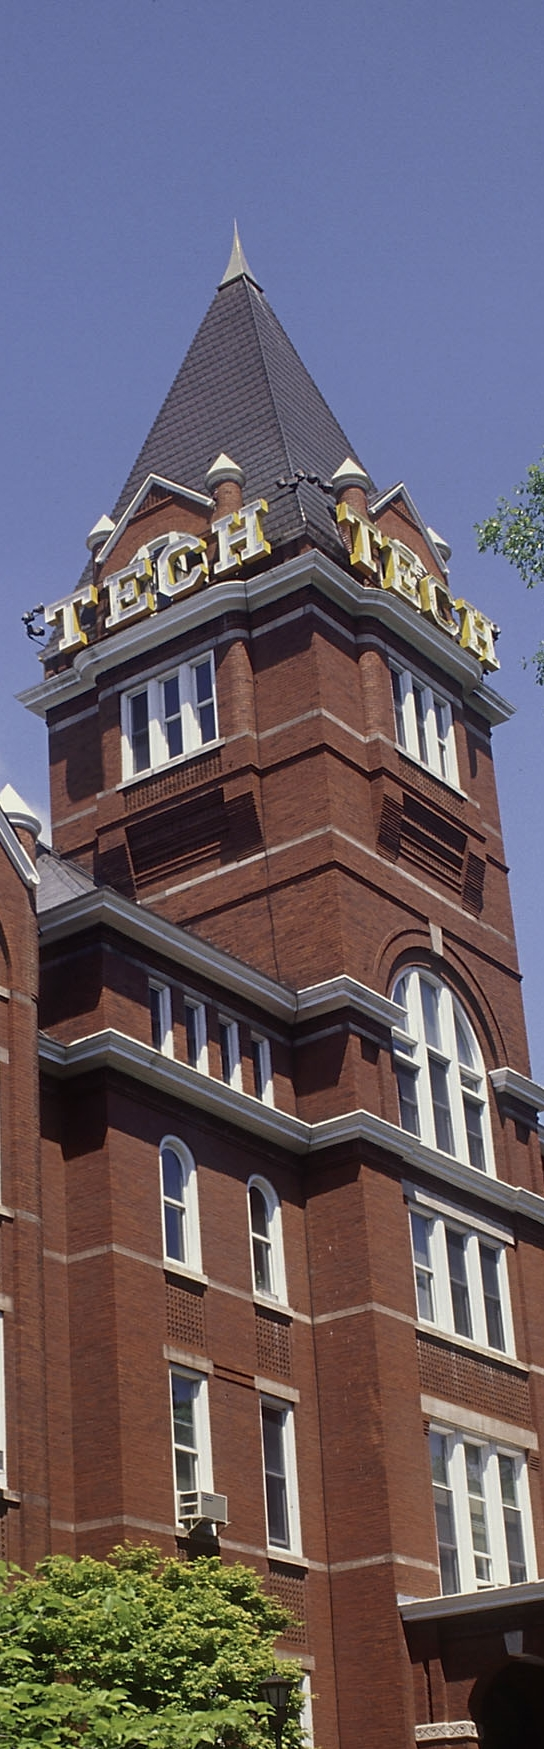
\includegraphics[width=1.25in]{figs/logo_TechTower.jpg}
    	\end{textblock}
    }

%logo tree
    \newcommand{\logoTree}
    {
    	\begin{textblock}{1}(0,0) 
    		\includegraphics[width=1.25in]{figs/logo_tree.jpg}
    	\end{textblock}
    }
%page numbers
    \newcommand{\mypagenum}
    {
    	\begin{textblock}{1}(1,94) 
		{\tiny \color[rgb]{0.2,0.2,1}\insertframenumber} %\insertframenumber,\insertpresentationendpage, \inserttotalframenumber
    	\end{textblock}
    }
%my footnote citation
	\newcommand{\myFootnoteCitation}[2]
	{
		\footnote{\tiny \citeauthor{#1}, \emph{#2}, \citeyear{#1}.}  %\citeauthor{#1}, \citetitle{#1}, #2 \citeyear{#1}.
	}
%my refer to citation
	\newcommand{\mycite}[1]
	{
		\emph{\citeauthor{#1} (\citeyear{#1})}
	}
%my footnote website citation
	\newcommand{\myFootnoteWebsiteCitation}[1]
	{
		\footnote{\tiny \citeauthor{#1}}
	}

\let\thefootnote\relax\footnotetext{Footnotetext without footnote mark}


%section underline
%\newcommand{\tmpsection}[1]{}
%\let\tmpsection=\section
%\renewcommand{\section}[1]{\tmpsection{\underline{#1}}}



%commands
	\newcommand{\likelihood}{p(Z_k| x_k) }						%likelihood
	\newcommand{\prior}{p(x_k)  } 								%prior
	\newcommand{\posterior} {p(x_k| Z_k)}						%posterior
	\newcommand{\prediction} {p(x_k| Z_{k-1})}					%prediction
	\newcommand{\update} {p(x_k|Z_k)}							%update
	\newcommand{\observations} {p(Z_k)}						%observations
	\newcommand{\prevobservations} {p(Z_{k-1})}				%previous observations
	\newcommand{\dxpk} {dx_{k-1}}							%dx_{k-1}
	\newcommand{\ChapKolm}{\int{p(x_k| x_{k-1})p(x_{k-1}|Z_{k-1})} \dxpk} %Chapman Kolmogorov

	%algorithm specific: JPDAF
	\newcommand{\likelihoodJPDAF}{p(Z_k| \chi, m, Z_{k-1}) }		%1. likelihood
	\newcommand{\priorJPDAF}{p(\chi|m, Z^{k-1}} 				%2. prior	
	\newcommand{\observationsJPDAF} {p(Z_k}					%3. observations
	\newcommand{\posteriorJPDAF} {p(\chi| Z_k)}					%4. posterior

%environments
	\newenvironment{changemargin}[2]
	{
	  	\begin{list}{}
		{
			\setlength{\topsep}{0pt}%
			\setlength{\leftmargin}{#1}%
			\setlength{\rightmargin}{#2}%
			\setlength{\listparindent}{\parindent}%
			\setlength{\itemindent}{\parindent}%
			\setlength{\parsep}{\parskip}%
		}
	  	\item[]
		}
		{\end{list}
	}
%figures

%colors
\definecolor{darkgreen}{rgb}{0,0.5,0}

%personal details
	\author{Salman Aslam}
	\institute{Advisor, Dr Christopher Barnes (ECE)\\Co-advisor, Dr Aaron Bobick (CoC)\\Georgia Institute of Technology}
	\date{}

\begin{document}
%####################################################################################################
\title{Math}
%####################################################################################################
\begin{frame}[plain]\logoTechTower
	\titlepage
\end{frame}

\begin{frame}
\frametitle{Outline}
\logoCSIPCPL\logoTechTower
	\setcounter{tocdepth}{1}	
	\tableofcontents
\end{frame}


%#######################################################################
\section{Abstract Algebra}
%#######################################################################
\begin{frame}
\frametitle{Abstract algebra}
\framesubtitle{}
\logoCSIPCPL\mypagenum\mypagenum
	\begin{itemize}
		\item A field of mathematics that studies algebraic structures such as
			\begin{itemize}
				\item groups
				\item rings
				\item fields
				\item modules
				\item vector spaces
				\item algebras
			\end{itemize}
		\item Now refers to the study of all algebraic structures
		\item Distinct from the elementary algebra taught in
	schools.  Elementary algebra
		\begin{itemize}
			\item teaches the correct rules for manipulating formulas
	and algebraic expressions involving real and complex numbers, and
	unknowns
		\item can be taken as an informal
	introduction to the structures known as the real field and
	commutative algebra.
		\end{itemize}
	\end{itemize}
\end{frame}



\begin{frame}
\frametitle{Spaces}
\framesubtitle{}
\logoCSIPCPL\mypagenum\mypagenum
	\begin{figure}
		\includegraphics[width=1.0\textwidth]{figs/Math_spaces.pdf}
	\end{figure}
\end{frame}


%========================================================================
\subsection{Group}
%========================================================================
\begin{frame}
\frametitle{Group}
\framesubtitle{}
\logoCSIPCPL\mypagenum\mypagenum
	A group is an algebraic structure consisting of 2 things:
	\begin{enumerate}
		\item a set
		\item an operation
	\end{enumerate}
	The set and the operation must satisfy the following 4 axioms:
	\begin{enumerate}
		\item closure
		\item associativity
		\item identity
		\item invertibility
	\end{enumerate}
	Examples
	\begin{itemize}
		\item (Z,+): integers under addition
	\end{itemize}
\end{frame}





%========================================================================
\subsection{Ring}
%========================================================================
\begin{frame}
\frametitle{Ring}
\framesubtitle{definition}
\logoCSIPCPL\mypagenum\mypagenum
	\begin{itemize} 
		\item A ring is an algebraic structure in which addition and multiplication are defined
		\item Alternately, a ring is an algebraic structure consisting of a set together with 2 binary operations (usually called addition and multiplication), where each operation combines 2 elements of the set to form a third element
		\item Also, a ring is a set $\mathbf{R}$ equipped with 2 binary operations $+:RxR \rightarrow R$ and $.: RxR \rightarrow R$
		\item To qualify as a ring, the set together with its 2 operations, $(R, +, .)$ must satisfy the 
\emph{ring axioms}
		\begin{enumerate}
			\item $(R, +)$ is required to be an \emph{abelian} group under addition
			\item $(R, .)$ is required to be an \emph{monoid} under multiplication
			\item The distributive laws must hold
		\end{enumerate}
	\end{itemize}
\end{frame}




\begin{frame}
\frametitle{Ring}
\framesubtitle{examples}
\logoCSIPCPL\mypagenum\mypagenum
	\begin{itemize} 
		\item set of integers, $\mathbf{Z}$, together with the usual properties of addition and multiplication
		\item set of real numbers, $\mathbf{R}$ equipped with the usual addition and multiplication
		\item Polynomials form a ring under addition and multiplication
	\end{itemize}
\end{frame}


\begin{frame}
\frametitle{Ring}
\framesubtitle{history}
\logoCSIPCPL\mypagenum\mypagenum
	\begin{itemize} 
		\item first arose from attempts to prove Fermat's last theorem, starting with Richard Dedekind in the 1880s
		\item Generalized and firmly established during the 1920s by Emmy Noether and Wolfgang Krull
	\end{itemize}
\end{frame}




%========================================================================
\subsection{Field}
%========================================================================
\begin{frame}
\frametitle{Field}
\framesubtitle{}
\logoCSIPCPL\mypagenum\mypagenum
	\begin{itemize}
		\item A field is an algebraic structure in which the operations of addition, subtraction, multiplication and division (except division by zero) may be performed, and the same rules hold which are familiar from the arithmetic of ordinary numbers.
		\item \textbf{Examples.}  $\mathbb{C}$ (complex numbers), $\mathbb{Q}$
(rational numbers), $\mathbb{R}$ (real numbers)
	\end{itemize}
\end{frame}


%========================================================================
\subsection{Vector Space}
%========================================================================
\begin{frame}
\frametitle{Vector space}
\framesubtitle{}
\logoCSIPCPL\mypagenum\mypagenum
	\begin{itemize}
		\item A vector space is a collection of vectors
		\item  It is a set on which two operations, (vector) addition and (vector) multiplication are defined
		\item The most familiar vector spaces are 2D and 3D Euclidean spaces
	\end{itemize}
\end{frame}


%========================================================================
\subsection{Algebra}
%========================================================================
\begin{frame}
\frametitle{Algebra}
\framesubtitle{}
\logoCSIPCPL\mypagenum\mypagenum
	\begin{itemize}
		\item An algebra over a field $\mathbb{K}$, or a $K$-algebra, is a vector space over $K$
		\item Let $K$ be a field, and let $A$ be a vector space over $\mathbb{K}$.  After some steps (to be added), you can show that $A$ is an algebra over a field.
		\item Field $\Rightarrow$ Vector space $\Rightarrow$ Algebra.
	\end{itemize}
\end{frame}

%========================================================================
\subsection{Continuity}
%========================================================================
\begin{frame}
\frametitle{Continuity}
\framesubtitle{}
\logoCSIPCPL\mypagenum\mypagenum
	\begin{itemize}
		\item $C(\Omega)$: set of all continuous functions with domain $\Omega$
		\item function $f$ if said to be of \emph{class} $C^k$ if the derivatives $f', f'', \ldots, f^{(k)}$ exist and are continuous
		\item Smooth: function $f$ if said to be of \emph{class} $C^\infty$ if it has derivatives of all orders
		\item $C^0$: consists of all continuous functions
	\end{itemize}
\end{frame}


%#######################################################################
\section{Combinatronics}
%#######################################################################
\begin{frame}
\frametitle{Combinatronics}
\framesubtitle{}
\logoCSIPCPL\mypagenum\mypagenum
	\begin{figure}
		\includegraphics[width=1.0\textwidth]{figs/Math_combinatronics.pdf}
	\end{figure}
\end{frame}

%#######################################################################
\section{Trigonometric relations}
%#######################################################################
\begin{frame}
\frametitle{Trigonometric relations}
\framesubtitle{}
\logoCSIPCPL\mypagenum\mypagenum
	\begin{figure}
		\includegraphics[height=0.9\textheight]{figs/math_trigRelations_productIntegration.pdf}
	\end{figure}
\end{frame}



%#######################################################################
\section{Series}
%#######################################################################
\begin{frame}
\frametitle{Geometric series}
\framesubtitle{}
\logoCSIPCPL\mypagenum\mypagenum
	\begin{figure}
		\includegraphics[width=1.0\textwidth]{figs/math_Series_geometric.pdf}
	\end{figure}
\end{frame}


\begin{frame}
\frametitle{Taylor series}
\framesubtitle{}
\logoCSIPCPL\mypagenum\mypagenum
	\begin{figure}				
		\includegraphics[width=1.0\textwidth]{figs/math_taylorSeries.pdf}
	\end{figure}
\end{frame}

%####################################################################################################
\section{Linear algebra}
%####################################################################################################
\begin{frame}
\frametitle{Dot product (Strang)}
\framesubtitle{}
\logoCSIPCPL\mypagenum\mypagenum
	\begin{figure}				
		\includegraphics[height=0.9\textheight]{figs/MT_projections.pdf}
	\end{figure}	
\end{frame}


\begin{frame}
\frametitle{Linear algebra}
\framesubtitle{defintions: vector spaces}
\logoCSIPCPL\mypagenum\mypagenum
	\begin{itemize}
		\item bunch of vectors such that,
		\item add any 2, and result is in the space
		\item multiply a vector by a constant, and result is in space
		\item i.e., linear combinations, $cS + dT$, are in space
	\end{itemize}
\end{frame}

\begin{frame}
\frametitle{\small{Gram Schmidt orthogonalization}}
\framesubtitle{}
\logoCSIPCPL\mypagenum\mypagenum
	\begin{figure}				
		\includegraphics[height=0.8\textheight]{figs/MT_gramSchmidtOrthogonalization.pdf}
	\end{figure}	
\end{frame}

\begin{frame}
\frametitle{Linear algebra}
\framesubtitle{column spaces}
\logoCSIPCPL\mypagenum\mypagenum
	\begin{itemize}
		\item linear combinations of all column vectors
		\item you can solve exactly $Ax=b$ when $b$ is in the column space of $A$
		\item can I throw away any columns and still get the same column space?
	\end{itemize}
\end{frame}




\begin{frame}
\frametitle{Linear algebra}
\framesubtitle{subspaces}
\logoCSIPCPL\mypagenum\mypagenum
	\begin{itemize}
		\item {\color{red} subspace}
			\begin{itemize} 
				\item a vector space inside a vector space		
			\end{itemize}
		\item {\color{red} subspace intersection}
			\begin{itemize}
				\item Subspaces $V$ and $W$, is $V \cap W$ a subspace?
				\item take a vector $S \in V$ and $S \in W$
				\item take another vector, $T \in V$ and $T \in W$
				\item linear combinations of $S$ and $T$, then $cS + dT \in V$ and $cS + dT \in W$
			\end{itemize}
	\end{itemize}
\end{frame}


\begin{frame}
\frametitle{Linear algebra}
\framesubtitle{matrix multiplication}
\logoCSIPCPL\mypagenum\mypagenum
	\begin{figure}				
		\includegraphics[width=1.0\textwidth]{figs/math_linearAlgebra_rowColMult.pdf}
	\end{figure}
\end{frame}


\begin{frame}
\frametitle{Linear algebra}
\framesubtitle{miscellaneous stuff}
\logoCSIPCPL\mypagenum\mypagenum
	\begin{figure}				
		\includegraphics[width=1.0\textwidth]{figs/math_linearAlgebra_points.pdf}
	\end{figure}
\end{frame}




\begin{frame}
\frametitle{Linear algebra}
\framesubtitle{pivots}
\logoCSIPCPL\mypagenum\mypagenum
	\begin{figure}				
		\includegraphics[width=1.0\textwidth]{figs/math_linearAlgebra_pivots.pdf}
	\end{figure}
\end{frame}

\begin{frame}
\frametitle{Linear algebra}
\framesubtitle{basis}
\logoCSIPCPL\mypagenum\mypagenum
suppose that $B=\{v_1, v_2, \ldots, v_n\}$ is a \\
{\color{darkgreen} subset of a vector space $V$ over a field $\mathbf{F}$} \\
\vspace{0.3in}
then $B$ is a basis if it satisfies the following 2 conditions:
	\begin{itemize} 
		\item {\small {\color{blue} linear independence property}, \\ 
 $\forall a_1, a_2, \ldots, a_n, a_1v_1 + a_2v_2 + \ldots + a_nv_n = 0$ iff $a_1=a_2=\ldots a_n=0$}
		\item {\small {\color{blue} spanning property}, \\
 for every $x$ in $V$, it is possible to choose $a_1, a_2, \ldots, a_n \in \mathbf{F}$ such that $x = a_1v_1 + a_2v_2 + \ldots + a_nv_n$}
\footnote{\tiny - $\mathbf{F}$ could be the real or complex numbers $\mathbf{R}$ or $\mathbf{C}$}
\footnote{\tiny - algebraically, a basis is set of independent vectors that span the space}
\footnote{\tiny - geometrically, a basis is a set of coordinate axes}
	\end{itemize}
\end{frame}



\begin{frame}
\frametitle{Linear algebra}
\framesubtitle{inner product}
\logoCSIPCPL\mypagenum\mypagenum
	\begin{itemize}
		\item for same dimensions, inner product is equal to trace of outer product
		\item for 2 vectors $A$ and $B$,
			\begin{equation*}
				\begin{array}{lll}				
					<A,B> 	&= A'B \\
							&= B'A \\
							&= \mbox{tr}(AB') \\
							&= \mbox{tr}((AB')') \\
							&= \mbox{tr}(BA')
				\end{array}
			\end{equation*}
	\end{itemize}
\end{frame}


\begin{frame}
\frametitle{Linear algebra}
\framesubtitle{special matrices: overview}
\logoCSIPCPL\mypagenum\mypagenum
	\begin{enumerate}
		\item {\color{red} symmetric}
			\begin{itemize}
				\item {\color{blue}positive definite} (all eigenvalues, all pivots, all sub-determinants positive)
			\end{itemize}
	\end{enumerate}
\end{frame}


\begin{frame}
\frametitle{Linear algebra}
\framesubtitle{special matrices: symmetric}
\logoCSIPCPL\mypagenum\mypagenum
	most important kind of matrix
	\begin{enumerate}
		\item eigenvalues: real (for real matrix)
		\item eigenvectors: perpendicular
			\begin{itemize}
				\item well, an identity matrix is symmetric
				\item but for it, all vectors are eigenvectors
				\item and not all vectors are symmetric
				\item but we do know that we have repeated eigenvalues
				\item and so a plane of eigenvectors
				\item and so we can choose perpendicular eigenvectors
			\end{itemize}
	\end{enumerate}
\end{frame}


\begin{frame}
\frametitle{Linear algebra}
\framesubtitle{factorizations: spectral theorem}
\logoCSIPCPL\mypagenum\mypagenum
	For a normal matrix (i.e. $A^TA=AA^T$), the canonical (also called normal or standard form) is a diagonal matrix
\end{frame}




\begin{frame}
\frametitle{Linear algebra}
\framesubtitle{factorizations: eigen-decomposition}
\logoCSIPCPL\mypagenum\mypagenum
	\begin{figure}
		\includegraphics[width=1.0\textwidth]{figs/math_linearAlgebra_eigenDecomposition.pdf}
	\end{figure}
\end{frame}

\begin{frame}
\frametitle{Linear algebra}
\framesubtitle{factorizations: SVD}
\logoCSIPCPL\mypagenum\mypagenum
	\begin{figure}
		\includegraphics[height=0.85\textheight]{figs/math_linearAlgebra_svd.pdf}
	\end{figure}
\end{frame}


\begin{frame}
\frametitle{Linear algebra}
\framesubtitle{factorizations: SVD (example)}
\logoCSIPCPL\mypagenum\mypagenum
	\begin{figure}
		\includegraphics[width=1.0\textwidth]{figs/math_linearAlgebra_svd_example.pdf}
	\end{figure}
\end{frame}


\begin{frame}
\frametitle{Linear algebra}
\framesubtitle{factorizations: LU}
\logoCSIPCPL\mypagenum\mypagenum
\end{frame}

\begin{frame}
\frametitle{Linear algebra}
\framesubtitle{factorizations: QR}
\logoCSIPCPL\mypagenum\mypagenum
\end{frame}






\begin{frame}
\frametitle{Linear algebra}
\framesubtitle{factorizations: Jordan}
\logoCSIPCPL\mypagenum\mypagenum
\end{frame}


\begin{frame}
\frametitle{Linear algebra}
\framesubtitle{factorizations: Schur}
\logoCSIPCPL\mypagenum\mypagenum
\end{frame}




\begin{frame}
\frametitle{Linear algebra}
\framesubtitle{factorizations: Cholesky}
\logoCSIPCPL\mypagenum\mypagenum
\end{frame}

\begin{frame}
\frametitle{Linear algebra}
\framesubtitle{factorizations: polar}
\logoCSIPCPL\mypagenum\mypagenum
\end{frame}



\begin{frame}
\frametitle{Linear algebra}
\framesubtitle{subspaces: $\mathbf{R}^2$ and $\mathbf{R}^3$}
\logoCSIPCPL\mypagenum\mypagenum
	\begin{figure}				
		\includegraphics[height=0.7\textheight]{figs/math_linearAlgebra_R2R3.pdf}
	\end{figure}
\end{frame}



\begin{frame}
\frametitle{Linear algebra}
\framesubtitle{subspaces: column and null spaces}
\logoCSIPCPL\mypagenum\mypagenum
	\begin{figure}				
		\includegraphics[width=1.0\textwidth]{figs/math_linearAlgebra_spaces.pdf}
	\end{figure}

\vspace{0.1 in}
{\color{red} null space}
\begin{itemize}
	\item if all the $b$'s are zero, then the $x$'s are in the null space, and every $x$ is orthogonal to every row
		\begin{itemize}
			\item so the null space is orthogonal to the row space
		\end{itemize}
\end{itemize}
\end{frame}


\begin{frame}
\frametitle{Linear algebra}
\framesubtitle{orthogonality: orthogonal matrix}
\logoCSIPCPL\mypagenum\mypagenum
	\begin{enumerate}		
		\item square
		\item real	
		\item rows are orthonormal (orthogonal unit vectors)
		\item columns are also orthonormal
		\item determinant is 1 or -1
			\begin{itemize}
				\item converse is not true, having a determinant of 1 or -1 is not a guarantee of orthogonality
			\end{itemize}
		\item transpose = inverse
		\item eigenvalues have complex modulus (absolute value) 1
			\begin{itemize}
				\item i.e. they lie on unit circle in complex plane
			\end{itemize}
	\end{enumerate}
\end{frame}





\begin{frame}
\frametitle{Linear algebra}
\framesubtitle{orthogonality}
\logoCSIPCPL\mypagenum\mypagenum
	\begin{itemize}				
		\item vectors
		\item subspaces
		\item bases
	\end{itemize}
\end{frame}



%####################################################################################################
\section{PDEs}
%####################################################################################################
\begin{frame}
\frametitle{PDEs}
\framesubtitle{heat equation}
\logoCSIPCPL\mypagenum
\end{frame}

\begin{frame}
\frametitle{PDEs}
\framesubtitle{wave equation}
\logoCSIPCPL\mypagenum
\end{frame}


\begin{frame}
\frametitle{PDEs}
\framesubtitle{laplace equation}
\logoCSIPCPL\mypagenum
\end{frame}



\begin{frame}
\frametitle{PDEs}
\framesubtitle{poisson equation}
\logoCSIPCPL\mypagenum
\end{frame}



%#######################################################################
\section{Optimization}
%#######################################################################
\begin{frame}
\frametitle{Optimization}
\framesubtitle{Linear Programming}
\logoCSIPCPL\mypagenum

\end{frame}

\begin{frame}
\frametitle{Optimization}
\framesubtitle{Non-linear Programming}
\logoCSIPCPL\mypagenum
\end{frame}


\begin{frame}
\frametitle{Optimization}
\framesubtitle{Quadratic Programming}
\logoCSIPCPL\mypagenum
\end{frame}



\begin{frame}
\frametitle{Optimization}
\framesubtitle{Convex optimization}
\logoCSIPCPL\mypagenum
\end{frame}


\begin{frame}
\frametitle{Optimization}
\framesubtitle{Combinatorial optimization}
\logoCSIPCPL\mypagenum
\end{frame}



\begin{frame}
\frametitle{Optimization}
\framesubtitle{Gradient descent}
\logoCSIPCPL\mypagenum\mypagenum
	\begin{itemize}\tiny
		\item {\color{red}Given:} training pairs $(x_j, y_j)$
		\item {\color{red}To find:} learn parameters $\theta_i$ of a machine that when given input $x_j$ produces output $y_j$
		\item {\color{red}Gradient Descent algorithm:} $\theta_i :=\theta_i + \alpha \frac{\partial J}{\partial \theta_i}$
	\end{itemize}
Example:
$\mbox{\fontsize{6}{8}\selectfont$
	\begin{array}{ll}
		h_{\theta} &= \theta_0 x + \theta_1 \sin(x) \\
		J&= [\theta_0 x_0 + \theta_1 \sin(x_0) - y_0]^2  + [\theta_0 x_1 + \theta_1 \sin(x_1) - y_1]^2\\
		\frac{\partial J}{\partial \theta_0} &= 2[\theta_0 x_0 + \theta_1 \sin(x_0) - y_0]x_0 +  2[\theta_1 x_1 + \theta_1 \sin(x_1) - y_1]x_1\\
		\frac{\partial J}{\partial \theta_1} &= 2[\theta_0 x_0 + \theta_1 \sin(x_0) - y_0]\sin(x_0) +  2[\theta_1 x_1 + \theta_1 \cos(x_1) - y_1]\sin(x_1)\\
\theta_0 &:= \theta_0 + \alpha \left[[\theta_0 x_0 + \theta_1 \sin(x_0) - y_0]x_0 +  [\theta_1 x_1 + \theta_1 \sin(x_1) - y_1]x_1\right]\\
\theta_1 &:= \theta_0 + \alpha\left[ [\theta_0 x_0 + \theta_1 \sin(x_0) - y_0]sin(x_0) +  [\theta_1 x_1 + \theta_1 \sin(x_1) - y_1]sin(x_1)\right]
	\end{array}
$}$

	\begin{itemize}\tiny
		\item The analytical form of the derivative has to be computed only once if we have an analytical equation for J
			\begin{itemize}\tiny
				\item plug in numbers for every iteration
			\end{itemize}			
		\item Otherwise, the gradient needs to be computed at every step
		\item Morever, in every iteration, you have to sum over all training examples
			\begin{itemize}\tiny
				\item computationally expensive if number of  training pairs $(x_j, y_j)$ is large
			\end{itemize}
		\item As we get closer to a local minimum, the gradient starts getting smaller, and the adjustments to $\theta$ automatically start getting smaller as well
	\end{itemize}
\end{frame}




\begin{frame}
\frametitle{Optimization}
\framesubtitle{lagrange multipliers}
\logoCSIPCPL\mypagenum
\myFootnoteWebsiteCitation{Wikipedia}
	\begin{figure}				
		\includegraphics[width=1.0\textwidth]{figs/math_optimization_lagrangeMultipliers.pdf}
	\end{figure}
\end{frame}



\begin{frame}
\frametitle{Optimization}
\framesubtitle{lagrange multipliers: example}
\logoCSIPCPL\mypagenum
	\begin{figure}				
		\includegraphics[width=1.0\textwidth]{figs/math_optimization_lagrangeMultipliersExample1.pdf}
	\end{figure}
\end{frame}


\begin{frame}
\frametitle{Optimization}
\framesubtitle{LP: simplex, primal dual}
\logoCSIPCPL\mypagenum
	\begin{itemize}
		\item When using the simplex method, the goal of 
			\begin{itemize}
				\item primal: achieve optimality
				\item dual: achieve feasability (non-negative and resource constraints satisfied)
			\end{itemize}
	\end{itemize}
\end{frame}



%#######################################################################
%####################################################################################################
%\bibliographystyle{ieee}
%\bibliography{c:/salman/work/writing/MyCitations}
\end{document}
%####################################################################################################

%#######################################################################
